\documentclass{article}
\renewcommand\refname{Referencias}
\renewcommand\contentsname{\'Indice de Conten\'ido}
\usepackage{graphicx}
\graphicspath{{IMG/}}
\usepackage{caption}
\usepackage{subcaption}
\usepackage{float}
\usepackage{listings}
\lstset{
 showstringspaces=false,
 tabsize=2,
 frame=single,
 numbers=left
}

\title{\textsc{Paradigmas y Lenguajes de Programaci\'on\\Trabajo Pr\'actico N\'umero 1\\-- Pr\'actica --}}
\author{Ulises C. Ramirez [uli.r19@gmail.com]\\H\'ector Chripczuk\\Ver\'onica Gonzalez}
\date{14 de Septiembre, 2018}

\begin{document}
\maketitle
\pagenumbering{gobble}
\newpage

\section*{C\'odigo}
Todo el c\'odigo que est\'e expresado en el documento como respuesta a alg\'un ejercicio esta contenido en la carpeta \texttt{PascalFC}, junto con el archivo \texttt{*.lst} y el correspondiente \texttt{*.obj}.\\

\section*{Versionado}
Para el corriente documento se est\'a llevando un versionado a fin de mantener un respaldo del trabajo y adem\'as proveer a la c\'atedra o a cualquier interesado la posibilidad de leer el material en la \'ultima versi\'on disponible.\\

\begin{center}
  \textsc{Repositorio}: \textit{https://github.com/ulisescolina/UC-PYLP/}
\end{center}

\hfill--\textsc{Ulises}
\tableofcontents
\pagenumbering{gobble}
\newpage

% === Inicio del Cuerpo del Documento === %
\pagenumbering{arabic}
\section{Instalaci\'on PascalFC}
\label{sec:pascalfc}
\textsc{Consigna}: \textbf{Investigar y describir como instalar el lenguaje PascalFC en su sistema operativo. Lectura recomendada por la c\'atedra: p\'agina del Ing. John Coppens, \textit{http://jcoppens.com/soft/pfc2}}.\\

\textit{Descripci\'on de la instalaci\'on}: la descripci\'on a brindar se realiza en una m\'aquina con las siguientes caracter\'isticas:\\

\begin{lstlisting}[caption={Caracter\'isticas sistema}]
~$ uname --kernel-name --kernel-release --machine
    --operating-system
Linux 4.15.0-34-generic x86_64 GNU/Linux
~$
\end{lstlisting}

para iniciar con la instalaci\'on se sigui\'o el v\'inculo a la p\'agina del Ing. John Coppens en el apartado de descargas [http://jcoppens.com/soft/pfc2/download.php], luego se procedi\'o a descargar la ultima versi\'on de la compilaci\'on del \texttt{pfc2}, que para el d\'ia 16 de Septiembre del 2018 es \texttt{pfc2-0.9.40.x86\_64.tar.gz}. Con el archivo comprimido descargado, solamente es necesario descomprimirlo en alguna carpeta que tengamos a mano, y despues de eso utilizar los dos archivos que son el resultado de la compilaci\'on del PascalFC, \texttt{pfc2} y el \texttt{pfc2int}, ah\'i tendremos el compilador e int\'erprete.\\

Finalizados estos pasos ya tendremos instalado el PascalFC, para la compilaci\'on y ejecuci\'on ser\'a necesario realizar en consola los siguientes pasos:

\begin{lstlisting}[caption={Compilaci\'on de y ejecuci\'on con pfc2}]
~$ cd /ruta/en/la/que/se/descomprimio/la/descarga/
~$ ./pfc2 archivo_a_ser_compilado.pfc
** Sucede la compilacion **
~$ ./pfc2int archivo_a_ser_compilado.obj
~$
\end{lstlisting}
\subsection{Pascal-FC + Geany}
De forma alternativa, se encontr\'o igualmente \'util la utilizaci\'on del manual ofrecido por la c\'atedra para la conjunci\'on del par de archivos que componen Pascal-FC (Compilador e Interprete) y el entorno de desarrollo Geany teniendo los mismos resultados satisfactorios que se logran en el manual.

\section{Codificaci\'on 1}
\label{sec:ej2}
\textsc{Consigna}: \textbf{Realizar un programa que ejecute paralelamente 2 procesos donde cada uno imprima por pantalla un numero ``ID'' de proceso}.\\

\lstinputlisting[language=Pascal, caption={TP1, Ejercicio 2}, label=tp1ej2]{PascalFC/tp1_ej2.pas}

Una cuesti\'on a tener en cuenta en el \texttt{Listing \ref{tp1ej2}} es  el hecho de que la funci\'on \texttt{writeln} no es at\'omica, y es muy probable que se encuentre con intercalamiento aun mas de lo que ocurre con la funcion \texttt{write}.

Alivianar un poco esta situaci\'on de intercalamiento en el ejercicio, \textit{sin el uso de sem\'aforos} es imprimiendo un parametro al lado del otro utilizando la funcion \texttt{write} como se demuestra a continuaci\'on:

\lstinputlisting[language=Pascal, caption={TP1, Ejercicio 2 (write)}, label=tp1ej2_2]{PascalFC/tp1_ej2_2.pas}

\section{Codificaci\'on 2}
\label{sec:ej3}
\textsc{Consigna}: \textbf{realizar un programa que ejecute paralelamente 3 procesos, 2 de los procesos deben imprimir 5 n\'umeros pares y el otro 10 n\'umeros pares.}

\lstinputlisting[language=Pascal, caption={TP1, Ejercicio 3}, label=tp1ej3]{PascalFC/tp1_ej3.pas}

Cabe mencionar que en el c\'odigo anterior tambi\'en se padece de un caso bastante grave de intercalaci\'on.

\section{Codificaci\'on 3}
\textsc{Consigna}: \textbf{crear un algoritmo que calcule todos los n\'umeros primos entre 1 y 100. Distribuir los datos para que cada proceso tome el mismo n\'umeor de elementos. ?`Es una distribuci\'on \'optima? Justifique.}

Antes de presentar el c\'odigo del programa se aclara que fue necesario el uso de sem\'aforos aunque el ejercicio no lo pida, para poder as\'i presentar la informaci\'on solicitada de manera legible, de otra manera no iba a ser discernible si la implementaci\'on paralela del algoritmo tuvo \'exito.

\lstinputlisting[language=Pascal, caption={TP1, Ejercicio 4}, label=tp1ej4]{PascalFC/tp1_ej4.pas}

\section{Codificaci\'on 4}
\textsc{Consigna}: \textbf{crear un algoritmo que realice el producto escalar de dos vectores de 10 elementos.}

\lstinputlisting[language=Pascal, caption={TP1, Ejercicio 5}, label=tp1ej5]{PascalFC/tp1_ej5.pas}

\section{Investigar}
\textsc{Consignas}: \textbf{
\begin{itemize}
  \item ?`Qu\'e diferencia existe entre la multiprogramaci\'on y el multiproceso?
  \item Describa que es una \textit{instrucci\'on at\'omica} y que es \textit{intercalacion}
  \item ?`Qu\'e son los sem\'aforos en la programaci\'on paralela? ?`Para qu\'e sirven?
  \item ?`Cu\'ales son sus instrucciones y para qu\'e se utiliza cada una?
\end{itemize}
}
\subsection{Multiprogramaci\'on y Multiproceso}
Ambos describen una forma de compartir el tiempo de computo de un sistema por programas, que en ultima instancia ayuda a dar una explicaci\'on conceptual de lo que significa concurrencia. La diferencia la expuesta en \cite{gortazarbellas} es la siguiente:
La \textbf{\textit{Multiprogramacion}}, se da cuando los programas se ejecutan en un \'unico procesador disponible y sus procesos internos comparten el tiempo de c\'omputo del procesador mencionado. Se habla de \textbf{\textit{Multiproceso}}, cuando el sistema en el cual se ejecuta el programa posee multiples procesadores, entonces es posible asignar diferentes procesos a diferentes procesadores.

\subsection{?`Qu\'e es una \textit{instrucci\'on at\'omica} y que es la \textit{intercalaci\'on}?}
\label{sub:atomicaintercalacion}
Se considera una \textit{instrucci\'on at\'omica} \cite{gortazarbellas} a aquella que se ejecuta completamente antes de que se ejecute ninguna otra instrucci\'on de cualquier otro proceso del programa, una \textit{intercalaci\'on} en un programa es una secuencia de ejecuci\'on de las instrucciones at\'omicas con las que cuente dicho programa, en el caso de que hayan 2 instrucciones at\'omicas ejecutadas por 2 procesos concurrentes, existiran 4 posibles intercalaciones.

\subsection{?`Qu\'e son los sem\'aforos en la programacion paralela?}
Los sem\'aforos son una herramienta que se destina para la sincronizaci\'on de procesos, en PascalFC estos son un tipo abstracto de datos, y como tal tiene operaciones y estructuras de datos internos. Todo sem\'aforo tiene un contador que toma valores positivos, y una lista de procesos asociados.
\subsection{?`Para qu\'e sirven?}
Estos sirven para garantizar que recursos en el sistema que deben ser utilizados por un proceso a la vez, efectivamente sean utilizados por un proceso a la vez, este conjunto de instrucciones que acceden a las areas mencionadas son denominados \textit{secci\'on cr\'itica}.

\subsection{?`Cuales son sus instrucciones y para que se utiliza cada una?}
Las operaciones que se pueden invocar sobre una variable de tipo sem\'aforo son:
\begin{itemize}
\item \texttt{initial(s,v)} inicializa el contador del sem\'aforo \texttt{s} al valor \texttt{v}. Este procedimiento solo se puede invocar una vez y debe ser llamado desde el programa principal. Debe ser inicializado antes de utilizarse.
\item \texttt{wait(s)} Este procedimiento solo se puede invocar desde un proceso. Funcionamiento:
  \begin{itemize}
    \item Si el contador \texttt{s} tiene un valor mayor que cero, el proceso contin\'ua su ejecuci\'on y el valor del contador se decrementa en uno.
    \item Si el contador del sem\'aforo tiene el contador igual a cero, el proceso se queda bloqueado y se a\~{n}ade a la lista de procesos bloqueados del sem\'aforo.
  \end{itemize}
\item \texttt{signal(s)} Este procedimiento solo se puede invocar desde un proceso. Funcionamiento:
  \begin{itemize}
    \item Si no hay procesos bloqueados en el sem\'aforo \texttt{s}, se incrementa el valor de contador en una unidad.
    \item Si hay procesos bloqueados en el sem\'aforo, se elige aleatoriamente a uno de ellos y se desbloquea para que continue su ejecuci\'on.
  \end{itemize}
\end{itemize}

\section{Aplicar sem\'aforos a los ejercicios en la \texttt{Secci\'on \ref{sec:ej2}} y la \texttt{Secci\'on \ref{sec:ej3}}}

\subsection{Ejercicio \texttt{Secci\'on \ref{sec:ej2}}}

\lstinputlisting[language=Pascal, caption={TP1, Ejercicio 2 (Sem\'aforo)}, label=tp1ej2s]{PascalFC/tp1_ej2_semaforo.pas}

\subsection{Ejercicio \texttt{Secci\'on \ref{sec:ej3}}}

\lstinputlisting[language=Pascal, caption={TP1, Ejercicio 3 (Sem\'aforo)}, label=tp1ej3s]{PascalFC/tp1_ej3_semaforo.pas}


\section{Inconvenientes de c\'odigo en el \texttt{Anexo \ref{sub:a11}}}

\textsc{Consigna}: \textbf{
\begin{itemize}
\item Explique brevemente las inconsistencias que posee el programa en el \texttt{Anexo \ref{sub:a11}}
\item Solucione el inconveniente utilizando sem\'aforos
\end{itemize}
}

\subsection{Inconsistencias en \texttt{Anexo \ref{sub:a11}}}
El segundo punto deja al descubierto el inconveniente mayor que posee el c\'odigo, el hecho que el ejercicio solicite que se solucione el problema con semaforos implica un caso de condicion de carrera en el acceso a la variable compartida \texttt{count}.\\

Ambos procesos estan compartiendo el espacio de memoria con la variable global mencionada y ninguno de los procesos asegura la manipulaci\'on de la misma mediante la solicitud de un cerrojo y consecuentemente tampoco se cede dicho cerrojo (lo cual tiene sentido porque no hay cerrojo que liberar), lo que hay que notar es que esto es un punto de inconsistencia en el programa. Esto causar\'ia problemas de inconsistencia con lo que ven los dos procesos, porque al momento de acceder cargar al registro, teniendo en cuenta que la operaci\'on de asignaci\'on no es at\'omica e involucra varios pasos los cuales se listan en la \texttt{Figura \ref{fig:asignacion}}, la variable para modificaci\'on en un proceso puede que tambien se este modificando en el otro lo que implicar\'ia que estar\'ia realizando uno de los pasos necesarios para la asignaci\'on, esto llevaria a que no se tome uno de los cambios, y por tanto se pierda informaci\'on.

\begin{figure}[H]
  \centering
  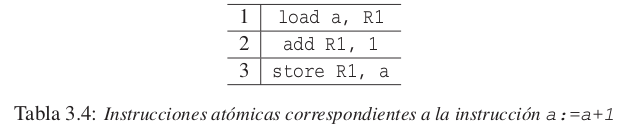
\includegraphics[width=.6\linewidth]{a+1.png}
  \caption{\cite{gortazarbellas}}
  \label{fig:asignacion}
\end{figure}

\newpage
\subsection{Solucion mediante sem\'aforos}

\lstinputlisting[language=Pascal, caption={TP1, C\'odigo de anexo (Sem\'aforo)}, label=tp1anexos]{PascalFC/tp1_anexo_semaforo.pas}

\section{Codificaci\'on 5}
\textsc{Consigna}: \textbf{escribir un algoritmo que posea 2 procesos, uno que produzca n\'umeros y los almacene en alg\'un tipo de estructura (\textit{investitar el tipo channel of}) y otro que tome los valores producidos y los imprima por pantalla. (Algoritmo productor-consumidor).}

Si bien encontr\'e algo, y con la similaridad con otras c\'atedras como Sistemas Operativos entiendo el concepto de que es lo que sucede en un algoritmo \textit{productor-consumidor}, no termino de entender el funcionamiento del codigo expresado en \cite{davies1992} que se lista a continuaci\'on.

\lstinputlisting[language=Pascal, caption={TP1, Productor-Consumidor \cite{davies1992}}, label=tppc]{PascalFC/tp1_prod-cons.pas}



% === Anexos === %
\newpage
\section{Anexos}

\subsection{Programa 1}
\label{sub:a11}
\lstinputlisting[language=Pascal, caption={TP1, C\'odigo de anexo}, label=tp1anexo]{PascalFC/tp1_anexo.pas}

% === Bilbiografia === %
\newpage
\begin{thebibliography}{99}
	% Item 1
	\bibitem[Gort\'azar Bellas, et al, 2012]{gortazarbellas}\textsc{Gort\'azar Bellas, Francisco; Mart\'inez Unanue, Raquel; Fresno Fern\'andez, Victor}. \textit{Lenguajes de Programaci\'on y Procesadores - Cap\'itulo 3.5}. Editorial Universitaria Ramon Areces, Madrid, 2012. \textsc{ISBN: 9788499610702}.
	% Item 2
	\bibitem[Davies, 1992]{davies1992}\textsc{Davies, G. L}. \textit{Pascal-FC: User guide for PC Compatibles}, Version 5, University of Bradford, UK, 1992.
\end{thebibliography}
\end{document}
